\section{Dominika Bujnarowska}
\label{sec:dominika}

Zdjęcie kota (see Figure~\ref{fig:cat})

\begin{figure}[htbp]
    \centering
    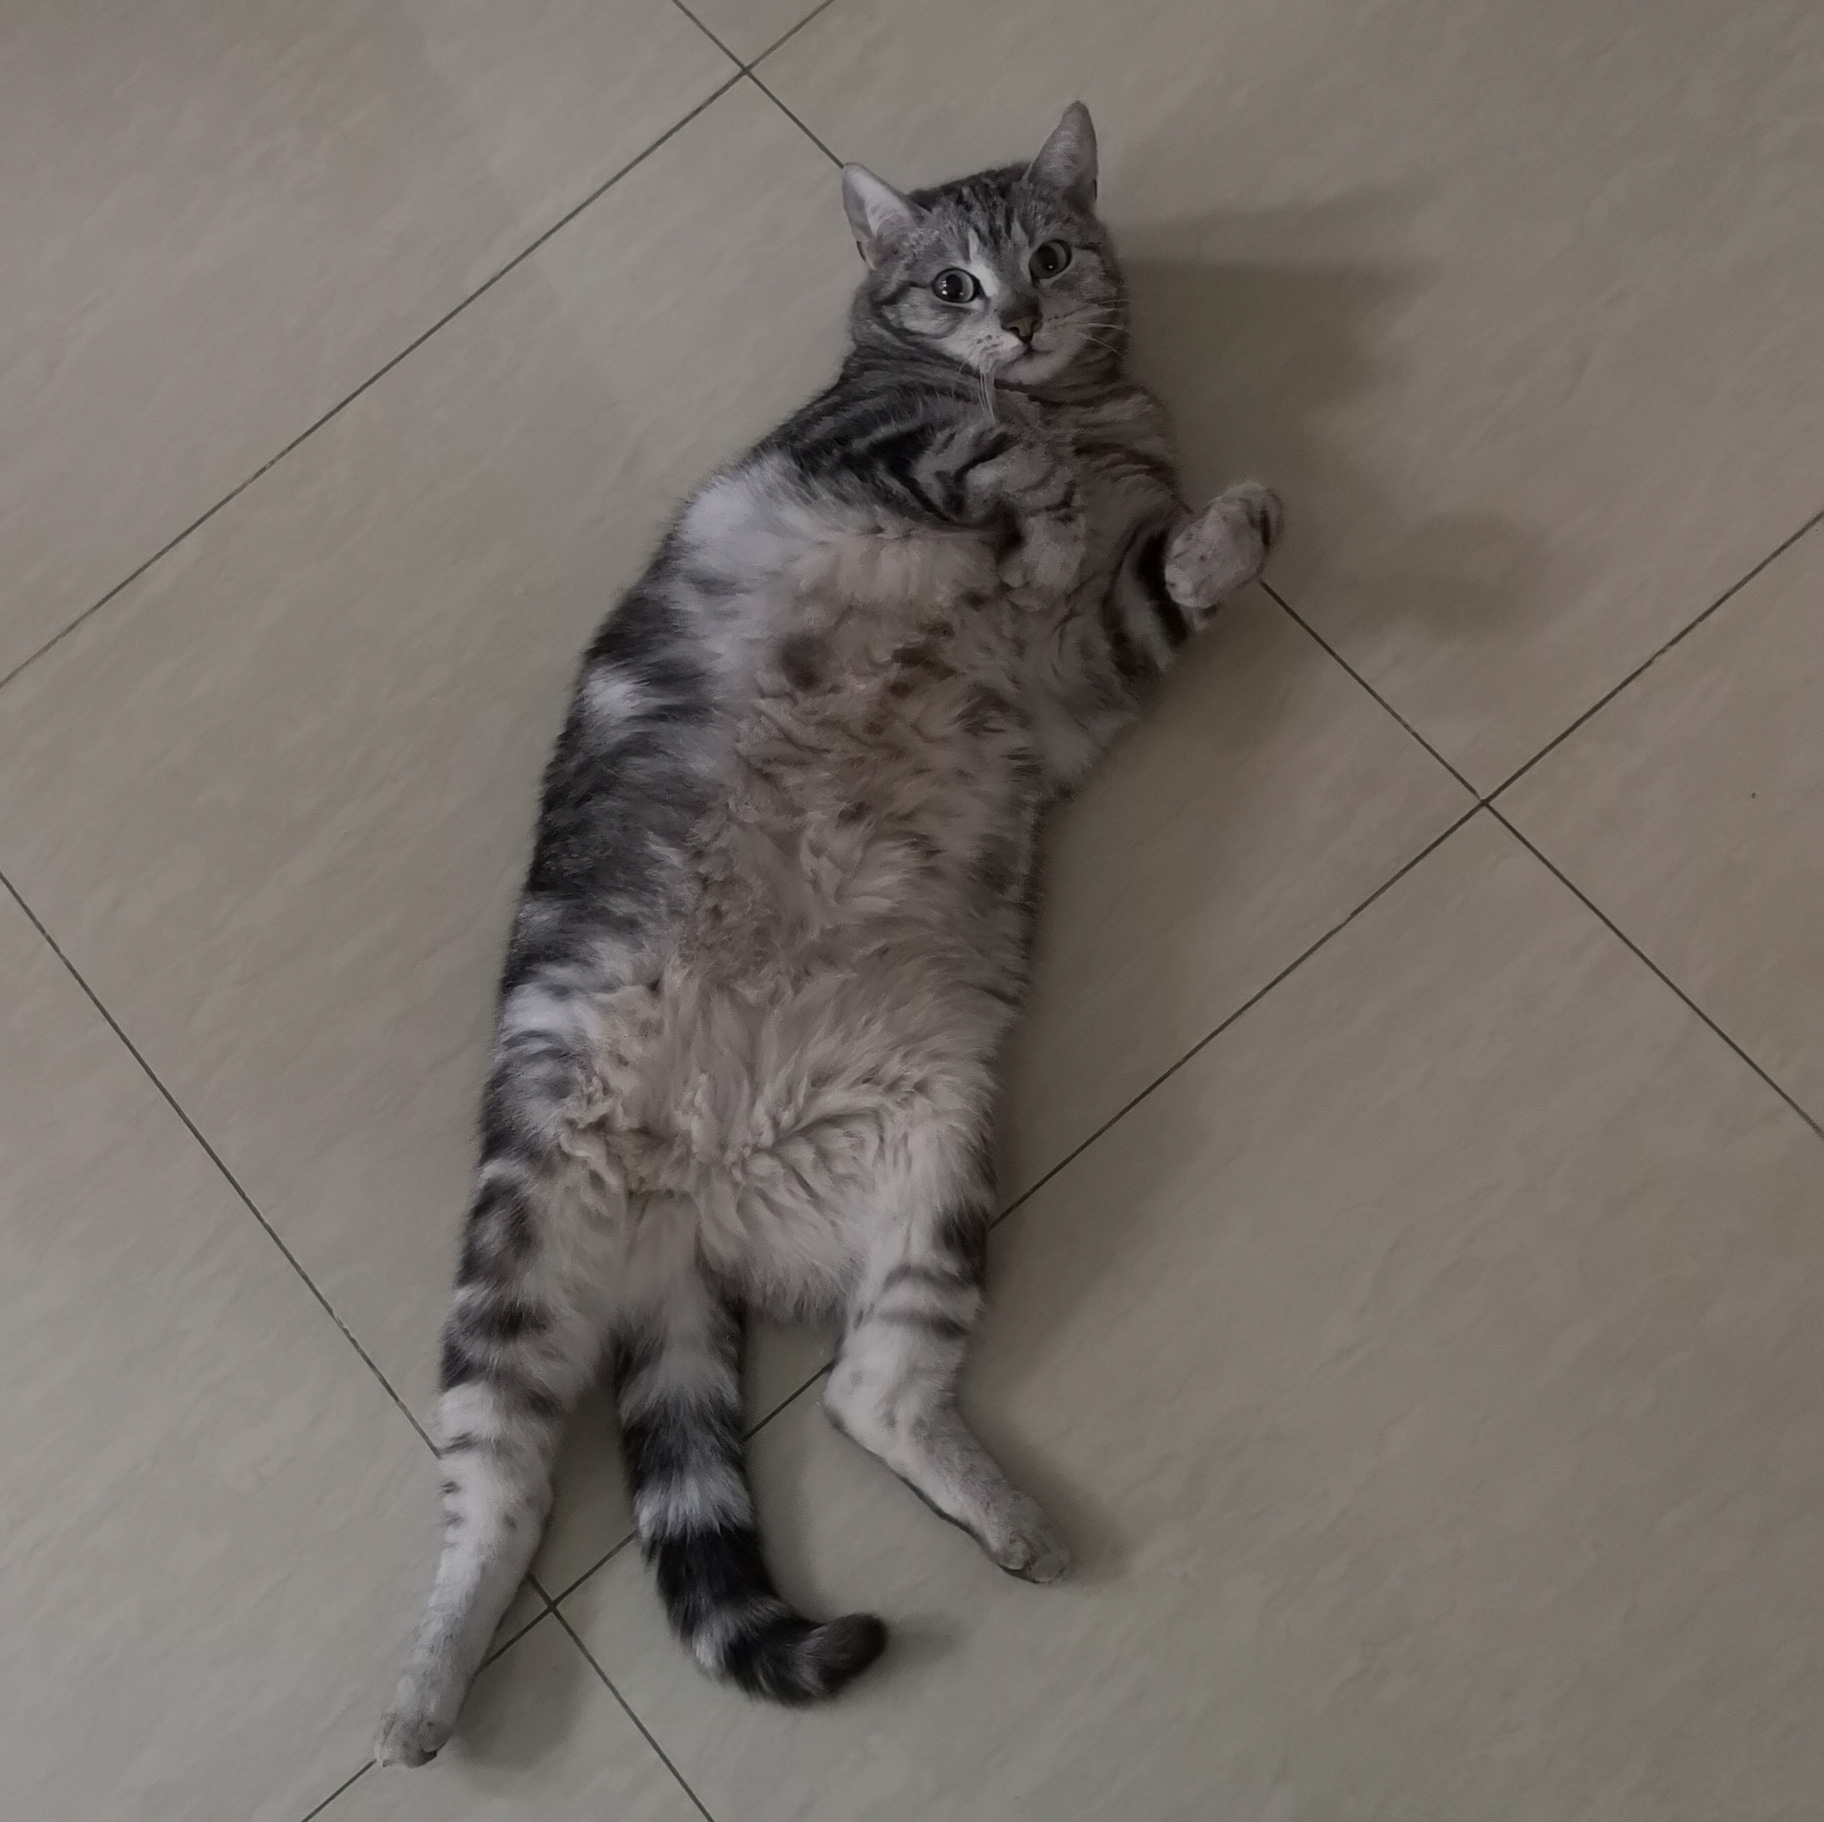
\includegraphics[width=0.25\textwidth]{pictures/dominika.jpg}
    \caption{To jest Lusia.}
    \label{fig:cat}
\end{figure}

Table~\ref{tab:liczby} Tabela z liczbami.
\begin{table}[htbp]
\centering
\begin{tabular}{|c|c|c|c|}
     \hline 
     Kolumna I & Kolumna II & Kolumna III & Kolumna IV \\ 
     \hline\hline
     1 & 2 & 3 & 4 \\ \hline
     10 & 20 & 30 & 40 \\ \hline
     100 & 200 & 300 & 400 \\ \hline
\end{tabular}
\label{tab:liczby}
\caption{Liczby w tabeli.}
\end{table}

Podstawowe wzory:
\[\int\cos(x)\,dx=sin(x)+c\]
\[\lim_{n\to\infty} \sqrt[n]{a} = 1\]

Numerowana lista:
\begin{enumerate}
    \item pierwszy item
    \item drugi item
    \item trzeci item
\end{enumerate}

Nienumerowana lista:
\begin{itemize}
    \item [-] pierwszy item
    \item [-] drugi item
    \item [-] trzeci item
\end{itemize}


\section*{Krótki tekst}
\textbf{'Cause} he gets up in the morning, and he goes to work at nine, and he comes back home at five-thirty, gets \underline{the same} train \textbf{\textit{every}} time. \par
\vspace{0.1cm}
\emph{'Cause} his world is built 'round punctuality it never fails.